%-------    CHAPTER 6     -------------------------------------------
%------ Interferometer Calibration ----------------------------------------
\chapter{Calibration}
\label{chap:cal}

\begin{figure}[!h]
\centerline{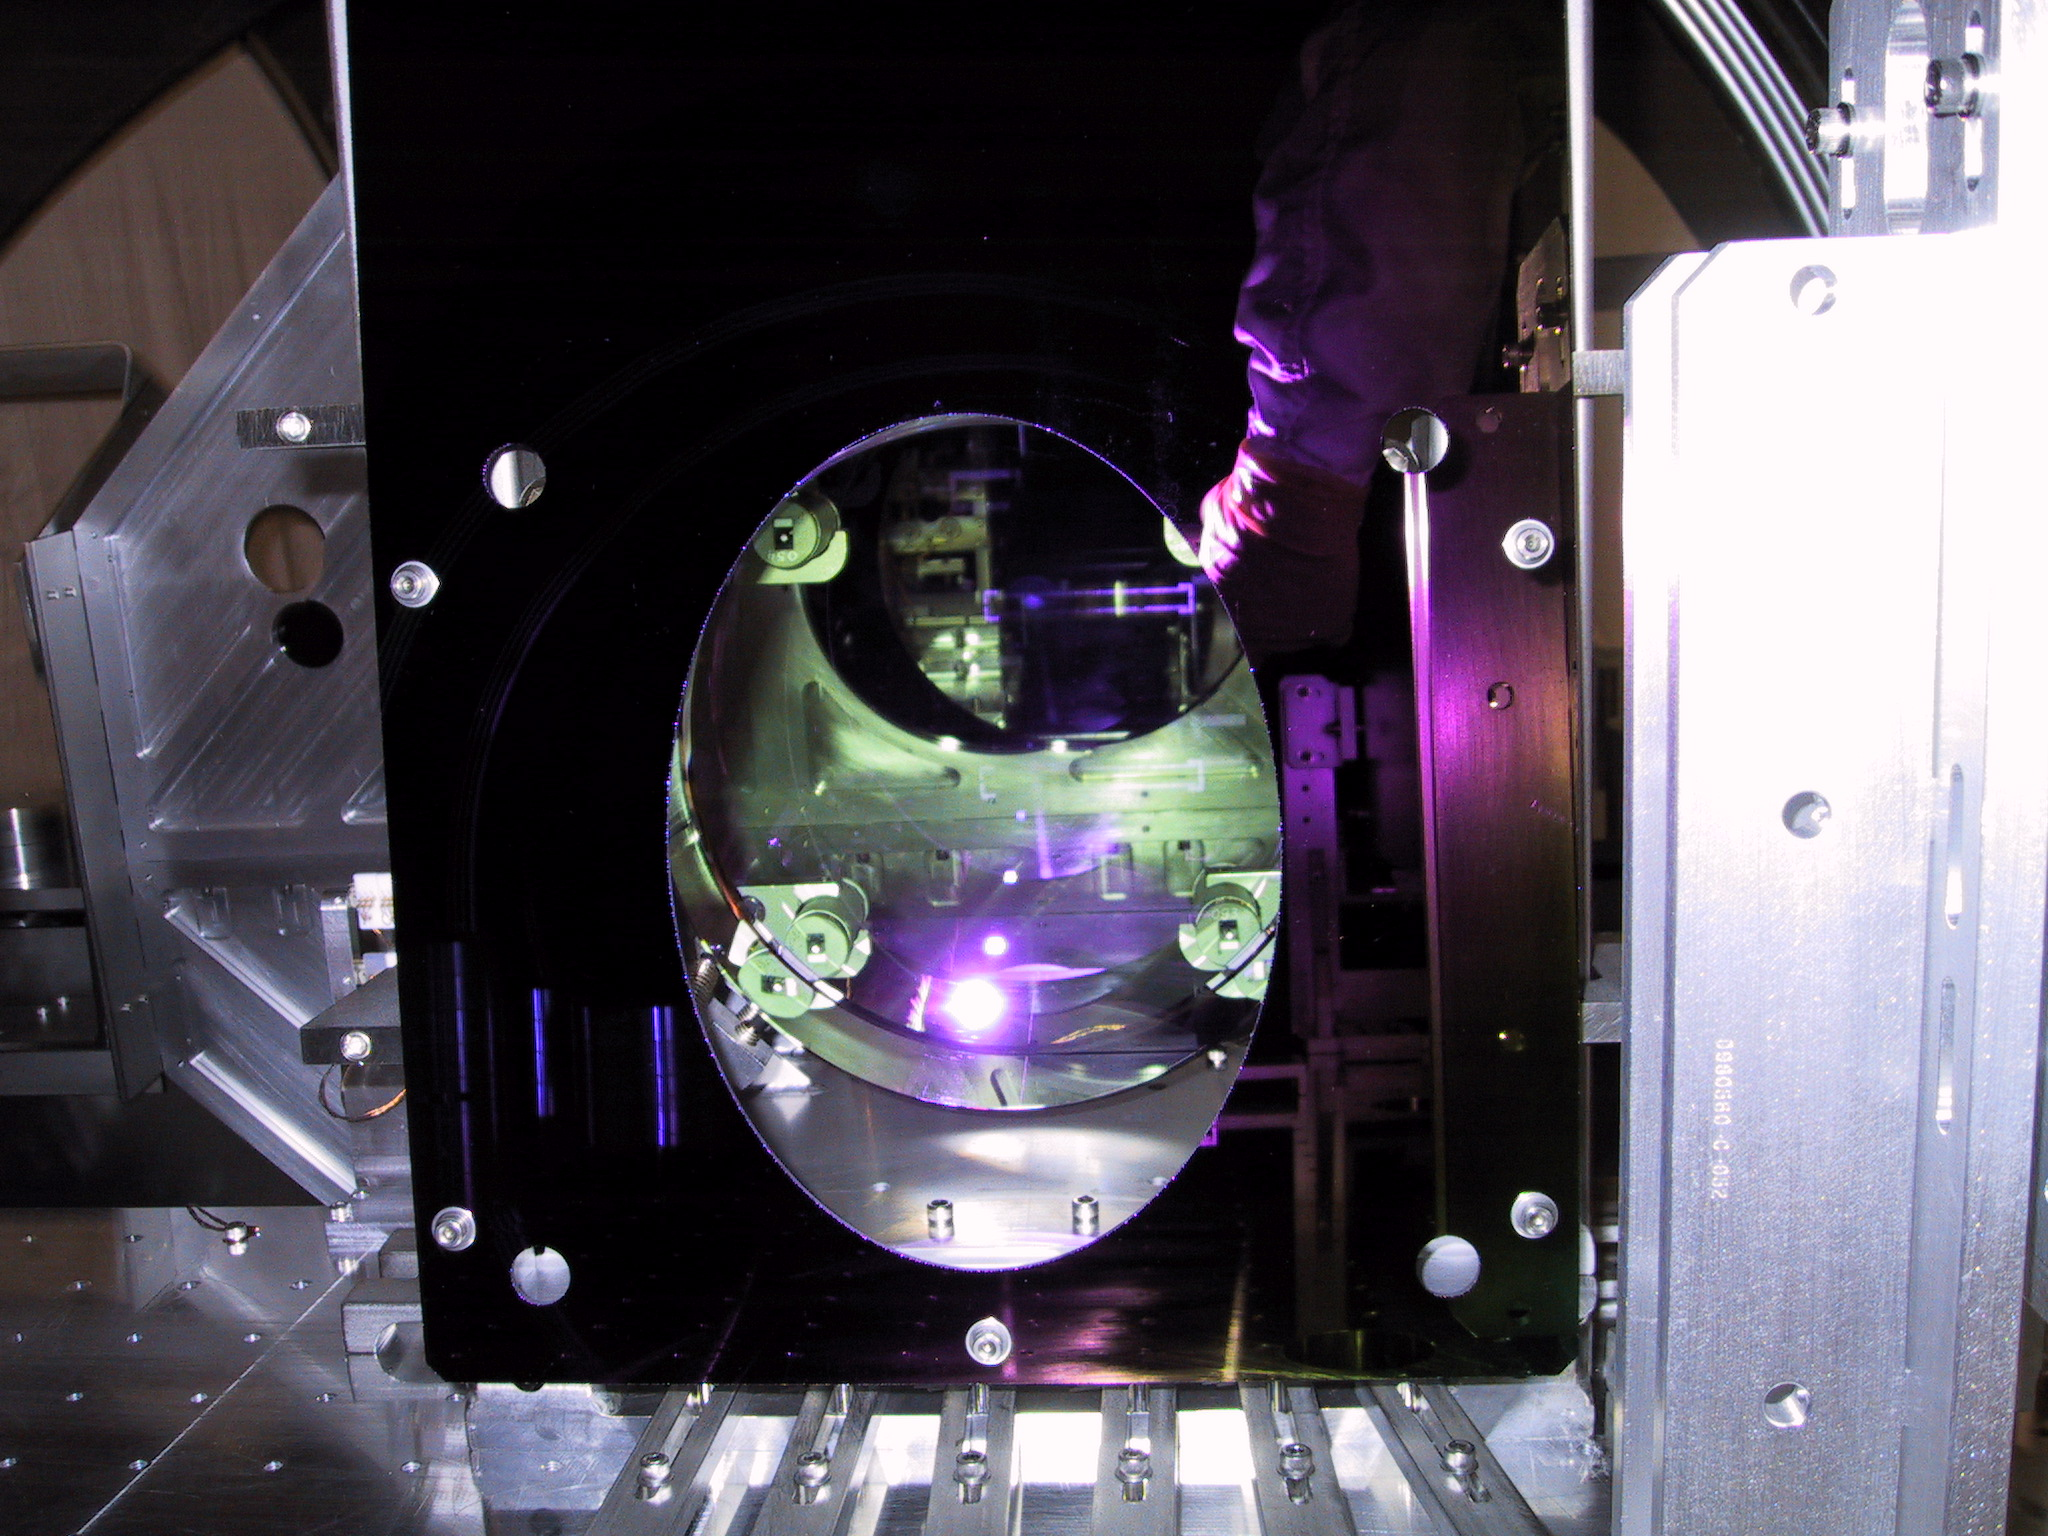
\includegraphics[angle=0,width=6.5in]{Figures/Chap6/RMfuckup.jpg}}
\end{figure}
\clearpage

This chapter describes how the interferometer's primary data channel is calibrated
to produce a measure of the gravitational wave strain incident on the 
detector~\cite{S1:Calibration,S2:Calibration}.

The interferometer output is a photocurrent which is proportional to the light power
modulation at the resonant sideband frequency ($\approx$25 MHz). We then turn this
into an integer time series after a series of analog signal conditioning
electronics. These inputs from multiple photodetectors and their electronics are
then further filtered digitally and then finally summed together to produce the
floating point time series used in the analyses. The name of the channel 
(L1:LSC-AS\_Q, H1:LSC-AS\_Q, or H2:LSC-AS\_Q) contains the following information:
the interferometer designation (L1, H1, or H2), the sub-system designation (Length
Sensing and Control), and the readout port and demodulation phase (AS port,
Quadrature phase).

This channel has the differential arm strain encoded in it. To properly decode 
this signal, 
we need to accurately determine the interferometer's \emph{response function}, 
defined as the function relating the data to the strain.


There are 3 major steps in calibrating the data:

\begin{itemize}

\item Make a model of the interferometer response (counts/meter).

\item Calibrate the mirror actuator drive (meters/count).

\item Track the calibration with a calibration line(s).
 
\end{itemize}

%------------------------------------------------------------------------------
\section{Interferometer Response Model}

The model of the interferometer's $L_-$ length control loop also serves to 
calculate the response of the DAQ channel (AS\_Q) to strains. 
Figure~\ref{fig:DARMmodel} shows a block diagram of the model and where in the
chain the data is extracted.

During standard interferometer operation, the 'Interferometer Optical Dynamics'
block, which represents the transfer function between strain and the optical
signal at the anti-symmetric port, is slowly varying (mainly due to interferometer
alignment variations).

During the S2 run, this fluctuation in the gain was uncompensated in the interferometer
control servos and led to instabilities and noise. In addition, these fluctuations
cause changes in the overall response function. Section~\ref{sec:CalLine} describes
how this is tracked.

\begin{figure}[!h]
\centerline{\includegraphics[angle=0,width=6in]{Figures/Chap5/DARM-model.png}}
\caption[L$_-$ Servo Model]{Block diagram of the model used to calculate the
         interferometer's response function. All analog circuit blocks have shadows.
         All digital blocks have orange borders.}
\label{fig:DARMmodel}
\end{figure}

The model outputs are all complex valued frequency domain transfer functions which
are supplied to all of the data analysis groups. The most commonly used product is
the response function, $R(f)$:

\begin{equation}
R(f) \equiv \frac{AS\_Q(f)}{Strain(f)}
\end{equation}


\section{Actuator Calibration}

To verify the response function given by the model, swept sine measurements are
made between the actuator and the readout in AS\_Q. To calibrate the actuator
we use the laser wavelength as the ultimate reference.

\subsection{Absolute Calibration}

A Michelson interferometer is a good displacement sensor. By misaligning the
end mirrors and the recycling mirror we get a Michelson interferometer made up
of the two arm cavity input mirrors (ITMX \& ITMY) and the beamsplitter (BS)
as shown in Figure~\ref{fig:Michelson}.

We lock the Michelson using the standard RF heterodyne readout of AS\_Q, but
limit the feedback bandwidth by putting an aggressive digital low-pass
filter in the servo loop. Then the AS\_Q signal is, in principle, directly
proportional to the differential length, $l_-$.

Since the actuator response is that of a damped pendulum with a 
$\simeq0.75$ Hz resonant frequency, it is well approximated as a
free mass in the band of interest (40-7000 Hz).

To get the absolute calibration, we have to calibrate AS\_Q in this configuration. 
To do this, we allow the mirrors to free
swing over several fringes. The peak-peak signal in AS\_Q corresponds
to a differential phase shift, $\phi_-$, of $\pi$, or correspondingly
a change in the position of a single arm mirror of $\lambda/4$, where
$\lambda = 1064$ nm, is the laser wavelength. 
So the AS\_Q calibration in ADC counts / meter is given by:

\begin{equation}
\mbox{AS\_Q cal} = \mbox{AS\_Q}_{pp}\frac{4 \pi}{\lambda} \frac{\mbox{ADC counts}}{\mbox{meter}}
\end{equation}
where this is meters of motion of a single mirror.

Systematic errors are continuously being eliminated and statistical errors
reduced through more patient measurement. The estimates on the S2 errors
are +/- 10\% in magnitude and phase~\cite{S2:Calibration}.


\subsection{Frequency Response}
To get the displacement response of the mirror to an actuation signal we measure 
the transfer function of each
piece of the mirror actuation chain shown in Figure~\ref{fig:OutputElectronics}. 
The digital compensation filters (''pre-DAC Whitening'' and 
''post-ADC un-whitening'' in Figure~\ref{fig:DARMmodel}) are constructed to
be exactly the inverse of their analog counterparts. This reduces the amount
of frequency dependent calibration error. The overall check is to again
measure the swept sine response of AS\_Q to the drive of a single mirror and
ensure that it faithfully follows the $f^{-2}$ power law of a free mass.


\section{Calibration tracking}
\label{sec:CalLine}

The variations in the interferometer optical gain are tracked by injecting a sinusoidal
drive into the digital control servo controlling the piston drive to one or both of
the arm cavity end mirrors. For the S2 run, three such calibration lines were injected 
in each interferometer: one at a low frequency ($\approx$50 Hz) where the servo 
loop gain is high, one at a frequency ($\approx$150 Hz) where the loop gain 
is $\approx$1, and one at a high frequency ($\approx$900 Hz) where the 
loop gain is low.

We use the actuator calibration to determine the amount the mirror is being
moved and monitor the amplitude and phase of the line in the data to get a 
measure of the interferometer response.



\section{Directions for the future}

There has been substantial progress in pinning down the absolute strain
calibration of the instruments and of tracking the calibration drift. The
following are some projects being pursued to further improve things:

\begin{itemize}
\item Optical gain fluctuations are currently tracked by the use of
      calibration lines and post-processing the data to correct for this. The
      real-time length control servos cannot afford such luxury, however.
      Instead, after S2, a dynamic digital gain correction was added. This
      system measures a few power levels in the interferometer and adjusts
      the digital gain in real time to correct the optical gain changes. In
      the future we should use the post-correction signal as our gravitational wave readout
      (this is the point just after the ''Input Matrix'' in Figures
       \ref{fig:DARMmodel} and \ref{fig:LSCscreen}).
      This should not only correct slow drifts in the calibration, but actually
      increase the measured strain sensitivity by removing bilinear upconversion
      from optical gain modulation at $\sim$1 second time scales.

\item The absolute calibration of the arm cavity end mirrors are now made by
      referencing them to the calibrated input mirrors. One can skip the
      intermediate step by directly referencing the end test mass drive
      to a laser wavelength shift. The laser frequency stabilization servo
      has a test input port (the AOM in Figure~\ref{fig:CMblock}) available
      for this purpose. The VCO can be directly calibrated against a spectrum
      analyzer or a high precision frequency counter.

\item It is possible to directly actuate the arm cavity mirrors through
      the radiation pressure force of an external laser. At 100 Hz, the
      displacement from a fully modulated 1 W laser at normal
      incidence is $\approx10^{-15}$ meters; quite a bit larger than
      what is currently used for a calibration line height. This radiation
      pressure calibration technique is a completely independent method to
      get the absolute calibration and avoids the complication of knowing 
      the analog filtering chain of the test mass actuators.
\end{itemize}





